\section{Introduction to Problem}
\paragraph*{}

Skin cancer is categorized into two types: melanoma and non-melanoma skin cancer. 
Melanoma, is the most dangerous kind of skin cancer accounted for an estimated 16,000 deaths 
each year from 2014 to 2016 in the United Kingdom (Cancer Research UK, 2020). 
The melanoma tumor caused by melanocytes can result in uncontrolled and abnormal growth which 
can spread in the human body \citep{KOROTKOV201269}.
Detection and classification of unknown pigmented skin lesions can result in early diagnosis 
of the medical problem. The research data provided by a cancer research organisation in 2017 has 
shown that melanoma was the 20th most common disorder with new incidents of 81,00 and 83,00 in males 
and females respectively in the United Kingdom \citep{KOROTKOV201269}. 
Dermoscopy is a non-invasive method of examining the pigmented skin, which includes microscopic imaging of the surface structure of pigmented
skin lesions \citep{KOROTKOV201269}.
Early diagnosis of pigmented skin lesions is crucial to classify skin disorders to decrease mortality concerning particular skin disorders. Dermoscopy improves the detection of melanoma compared to the detection of disease with naked eyes by analysing the pigmented skin lesion. Previous studies have shown that such tumours can result in higher chances of better treatment and cure of disease by removing the tumour \citep{CELEBI2007362}.
The current diagnosis method of detection involves using ABCD rule which considers the Asymmetry, Border irregularity, Colour irregularities, Darmascopic structures respectively of common pigmented skin lesions \citep{LOESCHER2013170}.
People working in busy work environments or less mobility can be victims of belated and slow diagnosis of such dangerous skin cancers.
The automated analysis of pigmented skin lesions using artificial neural networks can be beneficial in the optical analysis of microscopic images of pigmented skin lesions. 
The primary targeted audience who benefits from the outcome is the people who are working in busy work environments or people with less mobility are best to use cases that can use such an automated system. Booking a prior appointment with medical professionals based on the urgency of detected medical problems can result in the immediate treatment of patients with more critical conditions. The people with less mobility such as older audiences or people with special needs can detect pigmented skin lesions through online systems in an inconvenient manner. Medical institutions can use such technologies to automate the process of pre-health checkups and overcome the problem of shortage of staff members in case of emergency. Such automated systems can also result in the faster diagnosis of medical problems compared to a manual analysis by a clinician. 
Furthermore, manufacturing companies that supply the microscopic medical instruments can also use such intelligent models with their products to provide value to customers and medical institutions.

\section{Objective of Research}
The research concentrates on developing a type of artificial neural network called a convolutional network to perform automated optimal analysis to identify the class of pigmented skin lesions. 
The research focuses on providing the quantitative analysis on comparing the results predicted by the automated intelligent machine are compared with medical professionals to identify the classes of pigmented skin lesions. The study employs different experiments by applying different model architectures and analysing accurate hyper-parameters for optimal performance. 
The research concentrate on analyzing limited skin tumors such as melanoma, 
benign keratosis, melanocytic nevi and basal cell carcinoma. The hypothesis for the research is that the model will perform 
in same time efficient as the medical professionals in examining the pigmented skin lesions. The investigation employs publicly available HAM10,000 dataset \citep{DVN/DBW86T_2018}. 
The HAM10,000 dataset contains an extensive collection of 10,000 images of labelled data units that were collected from a diverse population of subjects over twenty years.
The outcome of the research project will analyse the effectiveness of the automated pigmented 
lesion system. Furthermore, the intelligent model will be deployed on a web-based system to provide an interface to use the system to analyse by the general audience.
\pagebreak

\section{Motivation and Targeted Audience}

Deep Learning technologies have always been fascinating for me to research on various models of neural networks. These artificial neural networks imitate the workings of the neural system and can be used as an intelligent system to recognise the visual patterns by analyzing the data. The primary motivation behind conducting the project is to research artificial neural networks to automate the optical classification tasks to help the community. The outcome of the research can be used by the general audience and healthcare institutions towards early diagnosis of common pigmented skin lesions. The secondary motivation behind developing such an automated deep learning system is to contribute towards reducing the mortality rates and improved pre-health checkup medical systems. An automated system can have an impact on the general audience by providing a convenient health checkup system which will detect melanoma and other common skin lesions.
The primary targeted audience who benefits from the outcome is the people who are working in busy work environments or people with less mobility are best to use cases which can use such an automated system. Booking a prior appointment with medical professionals based on the urgency of detected medical problems can result in the immediate treatment of patients with more critical conditions. The people with less mobility such as older audiences or people with special needs can detect pigmented skin lesions through online systems in an inconvenient manner. Medical institutions can use such technologies to automate the process of pre-health checkups and overcome the problem of shortage of staff members in case of emergency. Such automated systems can also result in faster diagnosis of medical problems compared to a manual analysis by a clinician. Furthermore, manufacturing companies which supply the microscopic medical instruments can also use such intelligent models with their products to provide value to customers and medical institutions. 

\pagebreak

\section{Perceptron Model}
\subsection{Inspiration from biological Structure of Neurons}
The human brain is composed of millions of specialised cell ”neurons” which are interconnected to each other, which carry electrical and chemical signals from neuron to another to function. 
There are an estimated 500 trillion connections between neurons in the human nervous system, which helps communicate signals \citep{patterson2017deep}.
The inspiration for artificial neural networks is taken from the functioning of the human brain and learn to recognise patterns and relationships in the data \citep{AGATONOVICKUSTRIN2000717}. 
\subsection{Neural Structure}
\vspace{3mm}
\begin{center}
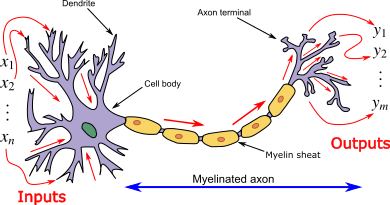
\includegraphics[width=10cm]{Images/neuron.png}
\end{center}

The figure above represents the biological structure of neurons that helps in the communication of electric signals in the nervous system to learn and process information. The biological structure of neurons
includes three major parts dendrites which are responsible for accepting the electrical and chemical signals to the neuron. 
Furthermore, the neuron contains the nucleus which is accountable for the processing input information with the neurons. 
At last, the processed information is passed to another neuron which is interconnected to neurons in the human nervous system through axon terminals
\citep{AGATONOVICKUSTRIN2000717}. 
 
\subsection{Perceptron Model}

\begin{center}
    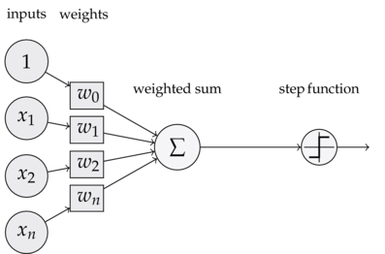
\includegraphics[width=0.6\textwidth]{Images/p_model.png} \\
\end{center}
\vspace{2mm}
Perceptron model was proposed by Frank Rosenblatt in 1943 to design the model to 
mimic the human brain \citep{939589}. Perceptron model or the single-layered feed forwards network 
networks take the vectors of inputs and multiply with a randomly 
initialized weights and add random bias to network and process the information by providing data to the
activation function to process the information \citep{AGATONOVICKUSTRIN2000717}.
The figure above represents the simple perceptron model which consists of inputs x and weights w 
for which the weighted sum of multiplication result of 
inputs and weights will be passed to the step activation function.

\subsection{Mathematical Representation }
\vspace{3mm}
{The equation below represents the preceptron model mentioned above in Mathematical notations.}
\begin{equation}
    \begin{split}
        y = \Big[\sigma(\sum_{k=0}^n x_k.w_k + b_k)\Big] \\
    \end{split}
\end{equation}

     {
        In, equation above ${\sigma = Activation function}$, x and w represents the inputs provided 
        and weights vectors in the network respectively. Furthermore, symbol b represents the bias in the equation, 
        during the optimization of the network weights and bias are adjusted accordingly to improve the predection. There are various activation functions ${\sigma}$ such as step function sigmoid, 
        relu, leaky relu and others that can be applied based on the requirements of the model prediction.
    }
\pagebreak
\section{Multi Layered Feed Forward Neural Network}
\begin{center}
    \begin{figure}[htp]
        \centering
        \begin{tikzpicture}[
        plain/.style={
          draw=none,
          fill=none,
          },
        dot/.style={draw,shape=circle,minimum size=3pt,inner sep=0,fill=black
          },
        net/.style={
          matrix of nodes,
          nodes={
            draw,
            circle,
            inner sep=8.5pt
            },
          nodes in empty cells,
          column sep=0.6cm,
          row sep=-11pt
          },
        >=latex
        ]
        \matrix[net] (mat)
        {
        |[plain]| \parbox{1cm}{\centering Input\\layer} 
                  & |[plain]| \parbox{1cm}{\centering Hidden\\layer} 
                               & |[plain]| \parbox{1cm}{\centering Output\\layer} \\
                  & |[plain]|                 \\
        |[plain]| &            & |[plain]|    \\
                  & |[plain]|  &              \\
        |[plain]| & |[dot]|                   \\
                  & |[plain]|  & |[dot]|      \\
        |[plain]| & |[dot]|    & |[plain]|    \\
        |[dot]|   & |[plain]|  & |[dot]|      \\
        |[dot]|   & |[dot]|    & |[plain]|    \\
        |[dot]|   & |[plain]|  &              \\
        |[plain]| &            & |[plain]|    \\
                  & |[plain]|                 \\
        };
        \foreach \ai/\mi in {2/I1,4/I2,6/I3,12/In}
          \draw[<-] (mat-\ai-1) -- node[above] {\mi} +(-1cm,0);
        \foreach \ai in {2,4,6,12}
        {\foreach \aii/\mii in {3/H1,11/Hn}
          \draw[->] (mat-\ai-1) -- (mat-\aii-2) node[yshift=0.6cm] {\mii};
        }
        \foreach \ai in {3,11}
        {  \draw[->] (mat-\ai-2) -- (mat-4-3);
          \draw[->] (mat-4-3) -- node[above] {O1} +(1cm,0);}
        \foreach \ai in {3,11}
        {  \draw[->] (mat-\ai-2) -- (mat-10-3);
          \draw[->] (mat-10-3) -- node[above] {On} +(1cm,0);}
        \end{tikzpicture}
        
        \caption{Multi Layered Neural Network diagram.}
        \label{fig_m_3}
        \end{figure}
\end{center}

The preceptron model acts the base for all the functioning of modern multi-layered neural networks.
The output of the single neuron described in the the above preceptron model is taken as the input in 
next layer of network. The above figure(1.1) shows an example of multi-layered neural where the first layer is known 
as input layer and intermediate layers are called hidden layer and last layer is known as output layer.
The single neuron can performe limited computation but the computation power increases with inter-connected
neurons in the network \citep*{AGATONOVICKUSTRIN2000717} where at each layer information is processed through the appropriate 
activation function. Artifical neural networks are designed to learn the patterns and relationships in the data  and 
requires enough amount of data to train and predict accurate outputs \citep*{AGATONOVICKUSTRIN2000717}.
The training data is passed to the neural network to recoganise the patterns in data and in each iteration or epoch 
the model predection gets improved with the optimisation algorithm which propagtes through the network to 
update the weights and bias to increase the accuracy.


\pagebreak
\subsection{Cost Function and Backpropagation Algorithm}
The objective for training deep learning models is to reduce
the error in prediction on each iteration and 
learn data patterns and relationships by increasing the 
prediction accuracy. Cost function is an appropriate method to 
analyse the performance of the neural network as it describes 
how well, model is predicting the actual results. The equation below 
describes the cost function equation also known as mean squared error \citep*{7013173}.
\vspace{2mm}

\begin{center}
\begin{equation}
    c = \frac{1}{2m} \sum_{i=1}^m(h - y)^2
\end{equation}
\end{center}

In, equation(1.2)  h is the predected outcome of the intelligent model 
and y is the actual value of the input. The equation above is mean square of 
predected value - actual value. The objective of optimisation algorithms is 
minimise the equation(1.2) to decrease the value of cost function so, the value is 
close to zero as much as possible so, that predected and actual 
value are almost same which means overall model accuracy has improved \citep*{7013173}. \\

The algorithm which aims to minimise the cost function is gradient descent. Gradient descent algorithm 
is a optimisation algorithm which is iterative in nature. 

\begin{center}
    \begin{equation}
            \frac{\partial }{\partial w} (\frac{1}{2m} \sum_{i=1}^m(h - y)^2)
    \end{equation}

    \begin{equation}
        \frac{\partial }{\partial b} (\frac{1}{2m} \sum_{i=1}^m(h - y)^2) 
    \end{equation}
\end{center}


The algorithm functions by finding the 
partial deravative of the cost function in respect to weights and bias as shown in the equation above.
The objective is to find minima of the cost fuction which improves the accuracy \citep*{7013173}. 
Backpropagation utilises the gradient descent algorithm and propgates after each layer to 
update the bias and weights in backwards direction to improve accuracy of the model. 